\documentclass[conference]{ieeetran}
\usepackage{amsmath,amssymb,amsfonts}
\usepackage{ucs}
\usepackage[utf8x]{inputenc}
\usepackage[english]{babel}
\usepackage[nottoc]{tocbibind}
\usepackage[left=2.5cm,right=2.5cm,top=2.5cm,bottom=2.5cm,]{geometry}
\usepackage{graphicx}
\usepackage{nameref}
\usepackage[hidelinks]{hyperref}
\usepackage{sidecap}
\usepackage{wrapfig}
\usepackage[bottom,hang]{footmisc} 
\usepackage{acronym}
\usepackage{multirow}
\usepackage{color}
\usepackage{capt-of}
\usepackage{array,			%better tables
			tabularx,			    %instead of tabular*             
			booktabs,			%tables for good publications
}
\usepackage{afterpage,hyperref} 
\usepackage{listings}
\usepackage{subfigure}


\begin{document}
\title{Seminar on Privacy in Ubiquitous Computing}

\author{\IEEEauthorblockN{Mehmed Mustafa}
\IEEEauthorblockA{\textit{Institute of Computer Science} \\
\textit{University of Göttingen}\\
mehmed.mustafa@stud.uni-goettingen.de}
\and
\IEEEauthorblockN{Chris Warin}
\IEEEauthorblockA{\textit{Institute of Computer Science} \\
\textit{University of Göttingen}\\
chris.warin@stud.uni-goettingen.de
}
}

\maketitle

\begin{abstract}
This document is a model and instructions for \LaTeX.
This and the IEEEtran.cls file define the components of your paper [title, text, heads, etc.]. *CRITICAL: Do Not Use Symbols, Special Characters, Footnotes, 
or Math in Paper Title or Abstract.
\end{abstract}

\begin{IEEEkeywords}
privacy, bystander, privacy enhancing technology
\end{IEEEkeywords}

\section{Introduction}
Today's society is filled with technological devices that are capable of gathering data from people, such as smartphones \cite{lu2017privacy}, surveillance cameras \cite{denning2014situ}, \ac{AR} devices \cite{shu2016cardea} or \ac{IoT} devices \cite{lu2017privacy}. Although these devices been causing a number of concerns regarding the privacy of users, another topic---that is less publicly discussed, but as important---is the privacy of bystanders, i.e. the people that are around users using these devices, and of which personal information can be collected without their knowledge or consent. A common real-life example could be a person taking a picture in a busy street, where the faces of bystanders are recognizable. The picture is taken without their knowledge nor consent, and can later be posted on social media. The data that are collected from bystanders can come from different mediums (i.e. pictures, videos, audio), and can be of different nature (i.e. face, voice, location). This results in pervasiveness in bystanders' privacy and touches several domains, namely economical, social, legal, and technological. This report focuses on the different technologies that address the pervasiveness in the privacy of bystanders. Section~\ref{BystandersPrivacy} lists different real-life examples of bystanders' privacy being compromised. Section~\ref{Technologies} goes over different technologies that ensure different aspects of the privacy of bystanders. Section~\ref{Limitations} describes the current limitations and challenges that these technologies are facing, whether they are technological or not. Finally, section~\ref{Conclusion} concludes this report.

\section{Bystanders’ privacy pervasiveness}\label{BystandersPrivacy}
Give real-life examples and why they are problematic.
\subsection{Videos and images}
Surveillance cameras, smartphone photos/videos in the street capturing bystanders
\subsection{Audio}
Google Home / Amazon Alexa in a household: other members are also listened
\subsection{Location}
Pervasive location information in apps (e.g. French StopCovid app recenses more contacts’ location information than announced)
\subsection{Others}
IoT, see example in 2.b

\section{Technologies for ensuring the privacy of bystanders}\label{Technologies}

\subsection{PriSurv Framework}
Reference \cite{chinomi2008PriSurv}

\subsection{Sharing of Multi-Subject and Interdependent Data}
Reference \cite{olteanu2018consensual}

\subsection{Cardea Framework}
Reference \cite{shu2016cardea}

\subsection{Others - More specific Audio or Location based technologies should be found}


\section{Limitations and challenges of privacy ensuring technologies}\label{Limitations}
\subsection{Cardea (user contribution)}
Willingly putting your personal data on a cloud to avoid having your privacy invaded by others can be seen as counter productive
\subsection{Example 2}
\subsection{Example 3}
\subsection{(optionally) Ideas that could fix these limitations}

\section{Conclusion}\label{Conclusion}


\begin{table}[htbp]
\caption{Table Type Styles}
\begin{center}
\begin{tabular}{|c|c|c|c|}
\hline
\textbf{Table}&\multicolumn{3}{|c|}{\textbf{Table Column Head}} \\
\cline{2-4} 
\textbf{Head} & \textbf{\textit{Table column subhead}}& \textbf{\textit{Subhead}}& \textbf{\textit{Subhead}} \\
\hline
copy& More table copy$^{\mathrm{a}}$& &  \\
\hline
\multicolumn{4}{l}{$^{\mathrm{a}}$Sample of a Table footnote.}
\end{tabular}
\label{tab1}
\end{center}
\end{table}

\begin{figure}[t]
\centerline{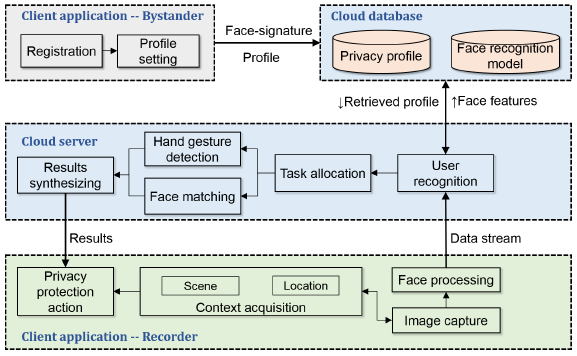
\includegraphics[width=.5\textwidth]{img/cardea_overview_diagram.png}}
\caption{Cardea framework overview.}
\label{fig}
\end{figure}


\section*{References}

Please number citations consecutively within brackets \cite{shu2016cardea}. The 
sentence punctuation follows the bracket \cite{dufaux2010framework}. Refer simply to the reference 
number, as in \cite{denning2014situ}---do not use ``Ref. \cite{denning2014situ}'' or ``reference \cite{denning2014situ}'' except at 
the beginning of a sentence: ``Reference \cite{lu2017privacy} was the first $\ldots$''

Number footnotes separately in superscripts.\cite{chinomi2008PriSurv} Place the actual footnote at 
the bottom of the column in which it was cited. Do not put footnotes in the 
abstract or reference list. Use letters for table footnotes.

Unless there are six authors or more give all authors' names; do not use 
``et al.''. Papers that have not been published, even if they have been 
submitted for publication, should be cited as ``unpublished'' \cite{lu2017privacy}. Papers 
that have been accepted for publication should be cited as ``in press'' \cite{olteanu2018consensual}. 
Capitalize only the first word in a paper title, except for proper nouns and 
element symbols.\cite{sen2016ipic}

For papers published in translation journals, please give the English 
citation first, followed by the original foreign-language citation \cite{olteanu2018consensual}.

\section*{Abbreviations and Acronyms}
\addcontentsline{toc}{section}{Abbreviations and Acronyms}
\begin{acronym}[Bash]
\acro{IoT} {\textit{Internet of Things}}
\acro{AR} {\textit{Augmented Reality}}
\end{acronym}

\bibliographystyle{ieeetr}
{\footnotesize
\bibliography{literature_list}}

\end{document}